\chapter{ Aufbau der optischen Diode}


Zur Vermeidung einer destabilisierenden Rückkopplung im He-Ne-Resonator setzen wir einen optischen Isolator ein, der in \cref{fig:function_of_optical_diode} dargestellt ist. 
Die Brewster-Fenster sind so angebracht, dass sie unter dem Brewster-Winkel \cite{introtoED}

\begin{equation}
  \tan\theta_B = \bigl(\tfrac{n_{\mathrm{glas}}}{n_{\mathrm{luft}}}\bigr),
\end{equation}
zur einfallenden Lichtwelle stehen, welches als erster Polarisationsfilter dient. 
Bei diesem Winkel durchquert p-polarisiertes Licht (elektrischem Feld in der Einfallsebene) die Glas-Luft-Grenzfläche nahezu ohne Reflexion, während s-polarisiertes Licht (Feld senkrecht zur Einfallsebene) teilweise reflektiert und somit unterdrückt wird. 
Dadurch ist der aus der Kavität austretende Strahl am Ausgangskoppler bereits stark linear entlang der p-Achse polarisiert und bietet somit einen wohldefinierten Eingangszustand für die nachfolgenden Isolator-Komponenten.

\begin{figure}[htbp]
  \centering
  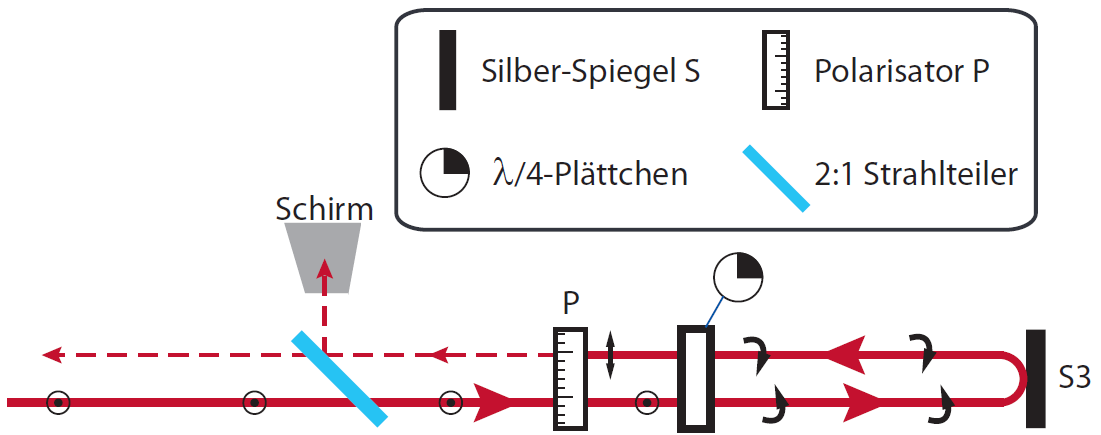
\includegraphics[width=0.75\linewidth]{Funktion der optischen Diode.png}
  \caption{Funktionsprinzip des optischen Isolators: Der rückwärts laufende Strahl ist zur Veranschaulichung leicht versetzt dargestellt. Schwarze Pfeile entlang des Strahlengangs zeigen mögliche Polarisationszustände in den einzelnen Stufen an. \cite{praktikum}}
  \label{fig:function_of_optical_diode}
\end{figure}

Der Isolator besteht aus einem linearen Polarisator (P), einer Viertelwellenplatte ($\lambda/4$) und einem reflektierendenSilber-Spiegel (S3), die unmittelbar hinter dem Ausgangskoppler in Serie angeordnet sind (siehe \cref{fig:aufbau_mit_optischer_diode}). 
Im Vorwärtsgang transmittiert der Polarisator ausschließlich p-polarisiertes Licht.
Dieses wird durch die $\lambda/4$-Platte in rechtszirkular polarisiertes Licht umgewandelt.
Nach der Reflexion an S3, welche die Drehrichtung der Polarisation beibehält, durchläuft das Licht erneut die $\lambda/4$-Platte, dies tritt als um 90° gedrehtes und wird dabei in s-polarisiertes Licht umgewandelt.
Dieses gedrehte Licht wird von P blockiert, sodass eine hohe nicht-reziproke Isolation erreicht wird, ohne nennenswerte Einfügedämpfung im Vorwärtsweg.

\begin{figure}[htbp]
  \centering
  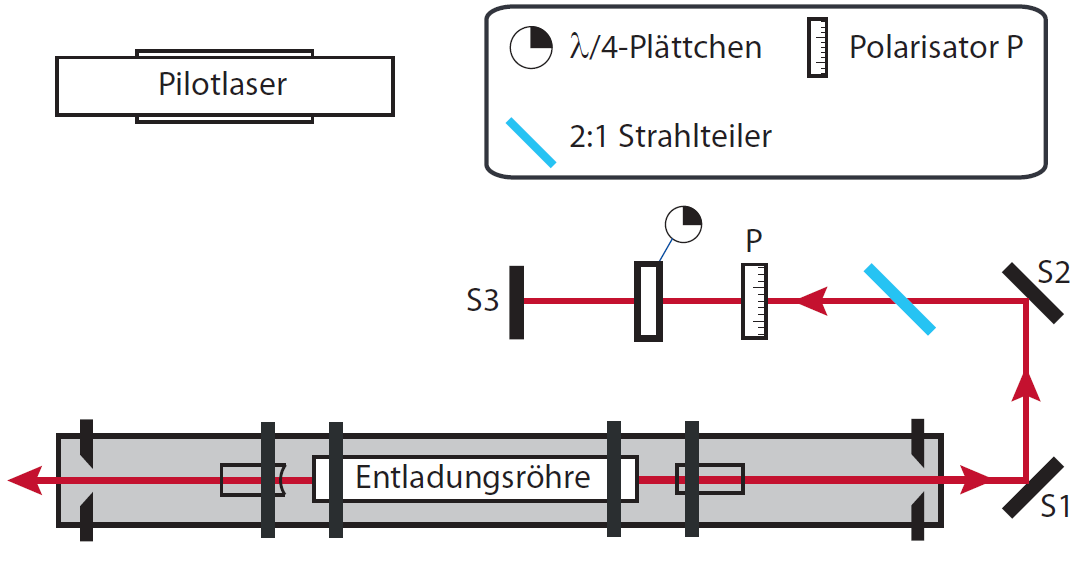
\includegraphics[width=0.75\linewidth]{Aufbau mit optischer Diode.png}
  \caption{Aufbau mit optischer Diode \cite{praktikum}}
  \label{fig:aufbau_mit_optischer_diode}
\end{figure}

Der Polarisator, die $\lambda/4$-Platte sowie ein nicht-polarisierender Strahlteiler (Verhältnis 2:1) sind in fein justierbaren Haltern montiert, welche axiale Ausrichtung sowie Kipp- und Drehbewegungen erlauben. 
Der Strahlteiler koppelt etwa ein Drittel des Vorwärtslichts zu einer photometrischen Leistungsüberwachung aus, während der verbleibende Anteil zur schnellen Photodiodenkette weitergeleitet wird. 
Alle optischen Elemente sind mit breitbandigen Antireflexbeschichtungen versehen, um unerwünschte Streureflexionen zu minimieren.

\paragraph{Justage-Prozedur:}
\begin{enumerate}
  \item \textbf{Polarisator-Orientierung:} Um die native p-Polarisation des Lasers einzustellen, wird P gedreht, bis die durch den Monitorport gemessene Leistung maximal ist.
  \item \textbf{Viertelwellenplatten-Einstellung:} S3 wird entfehrnt und  die $\lambda/4$-Platte justiert, bis die schwache Rückreflexion durch P auf einem Schirm verschwindet - dies ist ein Zeichen für eine perfekte 90°-Drehung der rücklaufenden Polarisation.
  \item \textbf{Isolations-Überprüfung:} S3 wird wieder eingesetzt und es wird geprüft, dass kein messbarer Rückfluss durch P auftritt, während die Vorwärtsdurchlässigkeit unverändert bleibt.  
\end{enumerate}

Während der Justage wurden der Polarisator auf einen Skalenwinkel von $\theta = 290^\circ \pm 1^\circ$ und die Viertelwellenplatte auf $\lambda/4 = 64^\circ \pm 1^\circ$ eingestellt.


%===============================================================================================================================================================================================================================================================================================================================================
\chapter{Optischer Spektrumanalysator} \label{sec:5.7}

Nach Verlassen des Isolators wird der He-Ne-Strahl in einen konfokalen Fabry-Perot-Resonator (\cref{fig:Spektrumanalysator}) mit äußerer Länge $l_{\mathrm{ext}} = 5{,}0\,\si{\centi\meter}$ eingekoppelt. \\
Die Eigenfrequenzen eines konfokalen Resonators ergeben sich laut Handbuch \cite{praktikum} zu
\begin{equation}
  \nu_{qnm}
  = \Bigl(q + \tfrac{m+n+1}{2}\Bigr)\,\frac{c}{2\,l} .
\end{equation}
wobei \( q \) der longitudinale und \( n, m \) die transversalen Modenzahlen sind. 
Gleiche transversale Moden TEM$_{nm}$ liegen damit im Abstand des freien Spektralbereichs
\begin{equation*}
  \Delta\nu_{\mathrm{FSR}}
  = \frac{c}{2\,l},
\end{equation*}
während benachbarte Moden um
\begin{equation*}
  \Delta\nu
  = \frac{c}{4\,l}
\end{equation*}
getrennt sind.
\begin{figure}[htbp]
  \centering
  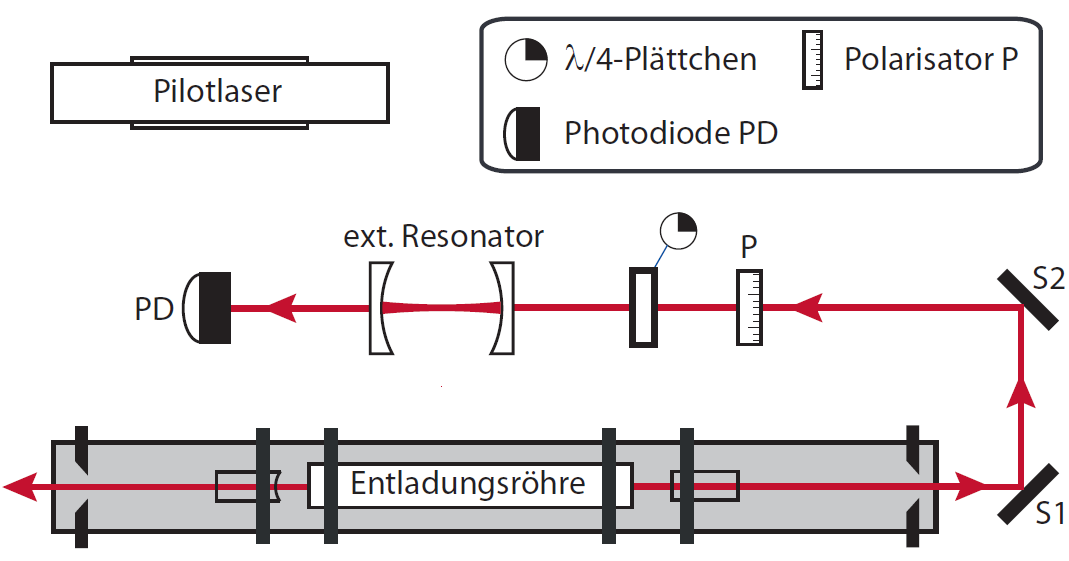
\includegraphics[width=0.75\linewidth]{Aufbaus zum optischen Spektrumanalysator.png}
  \caption{Schema des Aufbaus zum optischen Spektrumanalysator \cite{praktikum}}
  \label{fig:Spektrumanalysator}
\end{figure}
Ein Piezoaktor verändert \( l_{\mathrm{ext}} = 5{,}0\,\si{\centi\meter} \) um etwa \(200\,\si{\nano\meter}\) bei einer Dreiecksspannung von $0$–$100\,\si{\volt}$ bei $50\,\si{\hertz}$. 
Dadurch wird bei einem vollständigen Spannungszyklus exakt ein FSR überstrichen. 
Kanal 1 des Oszilloskops zeigt die Piezo-Spannung \( U(t) \), Kanal 2 die transmittierte Intensität \( I(t) \) einer langsamen Photodiode. 
Dies ergibt charakteristische Übertragungscluster, wie in den Abbildungen \cref{fig:9a} bis \cref{fig:9c} gezeigt.

Die Justage erfolgte mittels Papierziel und Zwei-Spiegel-Kippverfahren (\cref{fig:Resonator}). 
Eine korrekte Ausrichtung war erreicht, wenn bei jeder Piezo-Position ein einzelner scharfer Spot sichtbar war und die Übertragungspeaks minimal breit erschienen.
\begin{figure}[htbp]
  \centering
  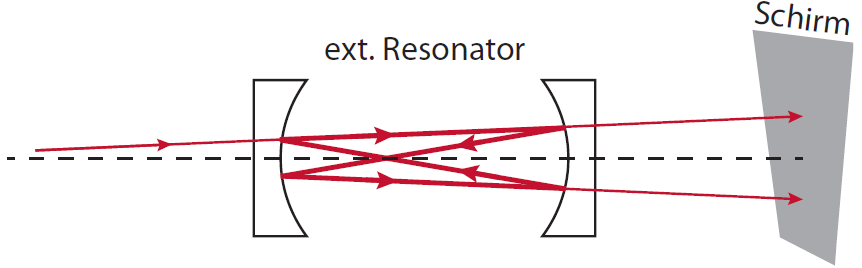
\includegraphics[width=0.75\linewidth]{Resonator bei Dejustage.png}
  \caption{Strahlengang im externen Resonator bei Dejustage \cite{praktikum}}
  \label{fig:Resonator}
\end{figure}
\begin{figure}[htbp]
    \centering
    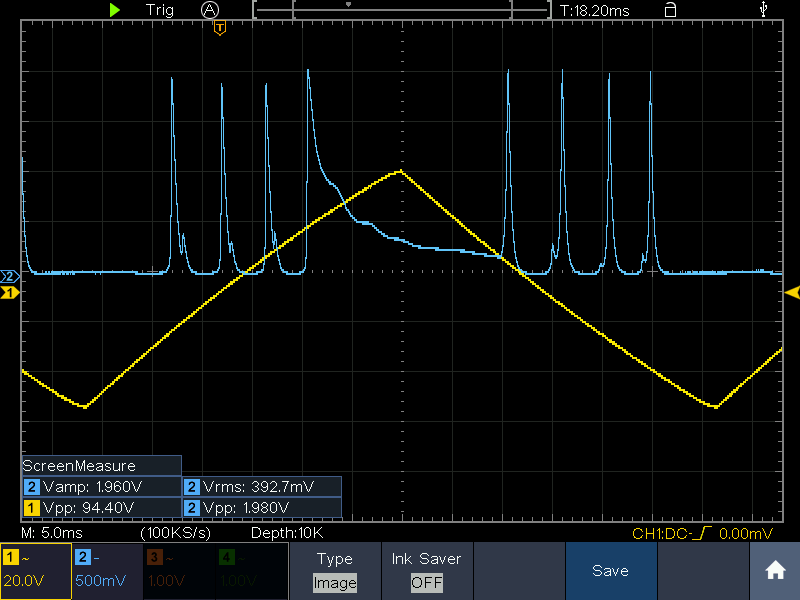
\includegraphics[width=0.75\linewidth]{52_1a.png}
     \caption{Oszilloskopübertragungscluster interne Kavitätenlängen $l = 52,0\,\si{\centi\meter} \pm$ 0{,}4\,\si{\centi\meter}.}
    \label{fig:9a}
\end{figure}
  \begin{figure}[htbp]
    \centering
    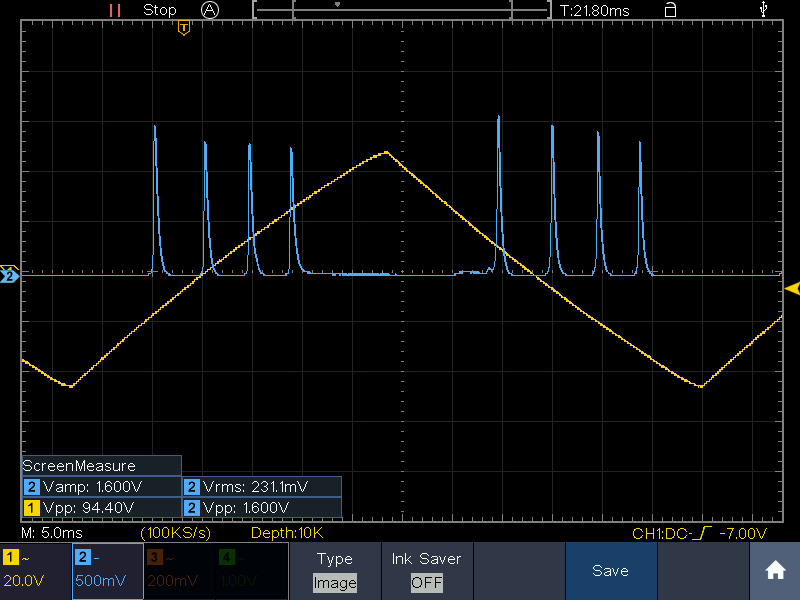
\includegraphics[width=0.75\linewidth]{68_1a.png}
     \caption{Oszilloskopübertragungscluste interne Kavitätenlängen $l = 68,0\,\si{\centi\meter} \pm$ 0{,}3\,\si{\centi\meter}.}
    \label{fig:9b}
  \end{figure}
  \newpage
  \begin{figure}[htbp]
    \centering
    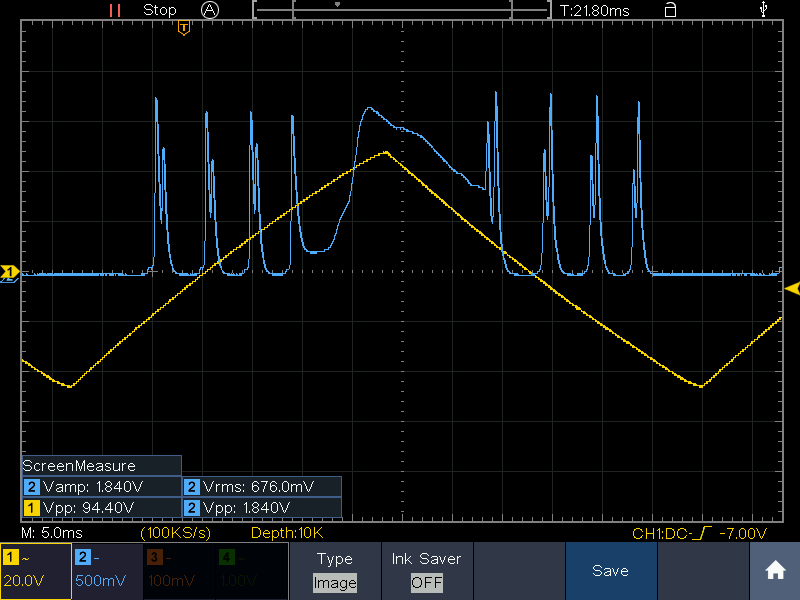
\includegraphics[width=0.75\linewidth]{80_1a.png}
     \caption{Oszilloskopübertragungscluster interne Kavitätenlängen $l = 80,0\,\si{\centi\meter} \pm$ 0{,}3\,\si{\centi\meter}.}
    \label{fig:9c}
  \end{figure}
 
 Für jede Oszilloskop-Spur bestimmen wir zwei Zeitintervalle: $a$, die horizontale Ausdehnung eines gesamten Übertragungsclusters (entspricht einer freien Spektralbreite des externen Fabry-Perot-Analysators), und $b$, der Abstand zweier benachbarter Peaks innerhalb dieses Clusters (entspricht dem longitudinalen Modenabstand der internen He-Ne-Kavität). 
 Da sowohl $a$ als auch $b$ auf derselben (möglicherweise nichtlinearen) Piezo-Zeitachse abgelesen werden, kompensiert ihr Verhältnis jede unbekannte Kalibrierkonstante. Damit lassen sich drei Frequenzintervalle definieren.

 Die freie Spektralbreite des Analysators beträgt:
\begin{equation}
  \Delta\nu_{\mathrm{FSR}}
  = \frac{c}{2\,l_{\mathrm{ext}}}
  = \frac{299\,792\,458\;\mathrm{m/s}}{2 \times 0{,}050\;\mathrm{m}}
  \approx 3{,}00\;\mathrm{GHz},
\end{equation}
wobei $l_{\mathrm{ext}} = 5{,}0\;\mathrm{cm}$.

Der experimentell bestimmte Modenabstand ergibt sich zu:
\begin{equation}
 \Delta\nu_{\mathrm{exp}}
  = \frac{b}{a}\;\Delta\nu_{\mathrm{FSR}},
\end{equation}

Mit der Fehlerfortpflanzung:
\begin{equation}
  \delta\Delta\nu_{\mathrm{exp}}
  =\Delta\nu_{\mathrm{exp}}
    \sqrt{\Bigl(\frac{\delta b}{b}\Bigr)^{2}
        + \Bigl(\frac{\delta a}{a}\Bigr)^{2}
        + \Bigl(\frac{\delta l}{l}\Bigr)^{2}}\!,
\end{equation}
wobei die Cursor-Unsicherheiten $\delta a = 0{,}20\;\mathrm{ms}$ und $\delta b = 0{,}20\;\mathrm{ms}$ sowie die Längenunsicherheiten $\delta l_{52} = 0{,}4\;\mathrm{cm}$ und $\delta l_{68} = \delta l_{80} = 0{,}3\;\mathrm{cm}$ betragen.

Der theoretische Modenabstand für eine ideale planparallele Kavität der Länge $l$ ist
\begin{equation}
 \Delta\nu_{\mathrm{theo}}
  = \frac{c}{2\,l},
  \quad
  \delta\Delta\nu_{\mathrm{theo}}
  =\Delta\nu_{\mathrm{theo}}\,\frac{\delta l}{l}.
\end{equation}

\begin{table}[H]
  \centering
  \resizebox{0.8\columnwidth}{!}{%
    \begin{tabular}{|c|c|c|c|c|}
      \hline
      $l \,\;\pm\delta l \,/\mathrm{cm}$ 
        & $a \,\pm \delta a\,/\mathrm{ms}$ 
        & $b \,\pm \delta b\,/\mathrm{ms}$ 
        & $v_{\mathrm{exp}}\pm\delta\Delta\nu_{\mathrm{exp}}\;/\;\mathrm{MHz}$ 
        & $v_{\mathrm{theo}}\pm\delta\Delta\nu_{\mathrm{theo}}\;/\;\mathrm{MHz}$ \\ \hline
      $52{,}0 \pm 0{,}4$   & $25{,}0 \pm 0{,}2$ & $3{,}0 \pm 0{,}2$ & $360 \pm 13$ & $288 \pm 2$ \\ \hline
      $68{,}0 \pm 0{,}3$   & $25{,}0 \pm 0{,}2$ & $2{,}0 \pm 0{,}2$ & $240 \pm 12$ & $220 \pm 1$ \\ \hline
      $80{,}0 \pm 0{,}3$   & $25{,}0\pm 0{,}2$ & $1{,}5 \pm 0{,}2$ & $180 \pm 12$ & $187 \pm 1$ \\ \hline
    \end{tabular}%
  }
  \caption{Experimentelle und theoretische Modenabstände für verschiedene interne Kavitätenlängen.}
  \label{tab:mode-spacings}
\end{table}

Der Modenabstand nimmt, wie theoretisch erwartet, proportional zu \(1/l\) ab. 
Für \(l = 68\,\si{cm}\) und \(l = 80\,\si{cm}\) stimmen die experimentellen Werte mit den theoretischen innerhalb der Fehlergrenzen überein, was sowohl die Kalibrierung des externen Resonators als auch die Anwendbarkeit der Formel \(\Delta\nu = c/(2l)\) auf die Laserresonatorlänge bestätigt. 
Die Abweichung bei \(l = 52\,\si{cm}\) um etwa 25\,\% ist vermutlich auf eine fehlerhafte Cursorplatzierung zurückzuführen (z.\,B. Wahl nicht-benachbarter Peaks oder falsche Bestimmung der Clustergrenze). 
Eine Wiederholung mit verbesserter Cursor-Positionierung dürfte hier Abhilfe schaffen.

Die Hauptunsicherheiten stammen von der Cursorplatzierung sowie der Längenbestimmung mit dem Maßband. 
Systematische Fehler wie Piezo-Hysterese oder Nichtlinearität des Sweeps kompensieren sich im Verhältnis \(b/a\), während verbleibende Justierfehler durch wiederholtes Feinkippen der Spiegel minimiert wurden.

Für zukünftige Verbesserungen wäre eine Digitalisierung der Oszilloskopspuren als CSV-Dateien empfehlenswert, um Lorentz-Fits durchzuführen. 
Diese könnten \(\delta a\) und \(\delta b\) auf unter \(0{,}02\,\si{ms}\) reduzieren. Zudem würde ein Messschieber mit Genauigkeit von \(\pm 0{,}05\,\si{cm}\) die relative Längenunsicherheit \(\delta l / l\) in den Bereich \(10^{-3}\) senken. 
Damit könnte die Gültigkeit des Gesetzes \(\Delta\nu \propto 1/l\) auf besser als 1\,\% bestätigt und die Kalibrierung des Spektrumanalysators noch exakter überprüft werden.

%===============================================================================================================================================================================================================================================================================================================================================
\chapter{ Präzise Messung des Modenabstandes mittels einer
optischen Schwebung} \label{sec:5.8}

Nach der spektralen Bestimmung des Modenabstands in \cref{sec:5.7} wird dieselbe Größe nun auf einer absoluten RF-Skala gemessen, indem zwei longitudinale Moden auf einer schnellen Photodiode interferiert werden. 
Das entstehende Differenzfrequenz-Signal im Hochfrequenzbereich (RF) wird anschließend mit einem 350\,MHz-Oszilloskop analysiert (\cref{fig:difffreq}). 
Zwei benachbarte Kavitätsfrequenzen $\nu_{1} = \omega_{1}/2\pi$ und $\nu_{2} = \omega_{2}/2\pi$ erzeugen nach quadratischer Detektion einen RF-Term bei der Differenzfrequenz


\begin{equation*}
  \Delta\omega = \omega_{1} - \omega_{2} = 2\pi\,\Delta\nu_{\mathrm{beat}},
\end{equation*}
wobei alle hochfrequenten Summen- und $2\omega$-Terme oberhalb der 35\,MHz-Tiefpassgrenze des Detektors liegen und somit unterdrückt werden. 
Die ganze Zahl $m$ bezeichnet die Anzahl der longitudinalen Intervalle zwischen den beiden Moden ($m=1$ für benachbarte Moden, $m=2$ für jeden zweiten Modenabstand usw.), sodass gilt
\begin{equation}
  \Delta\nu_{\mathrm{beat}} = m\,\Delta\nu_{\mathrm{laser}}.
\end{equation}

\begin{figure}[htbp]
    \centering
    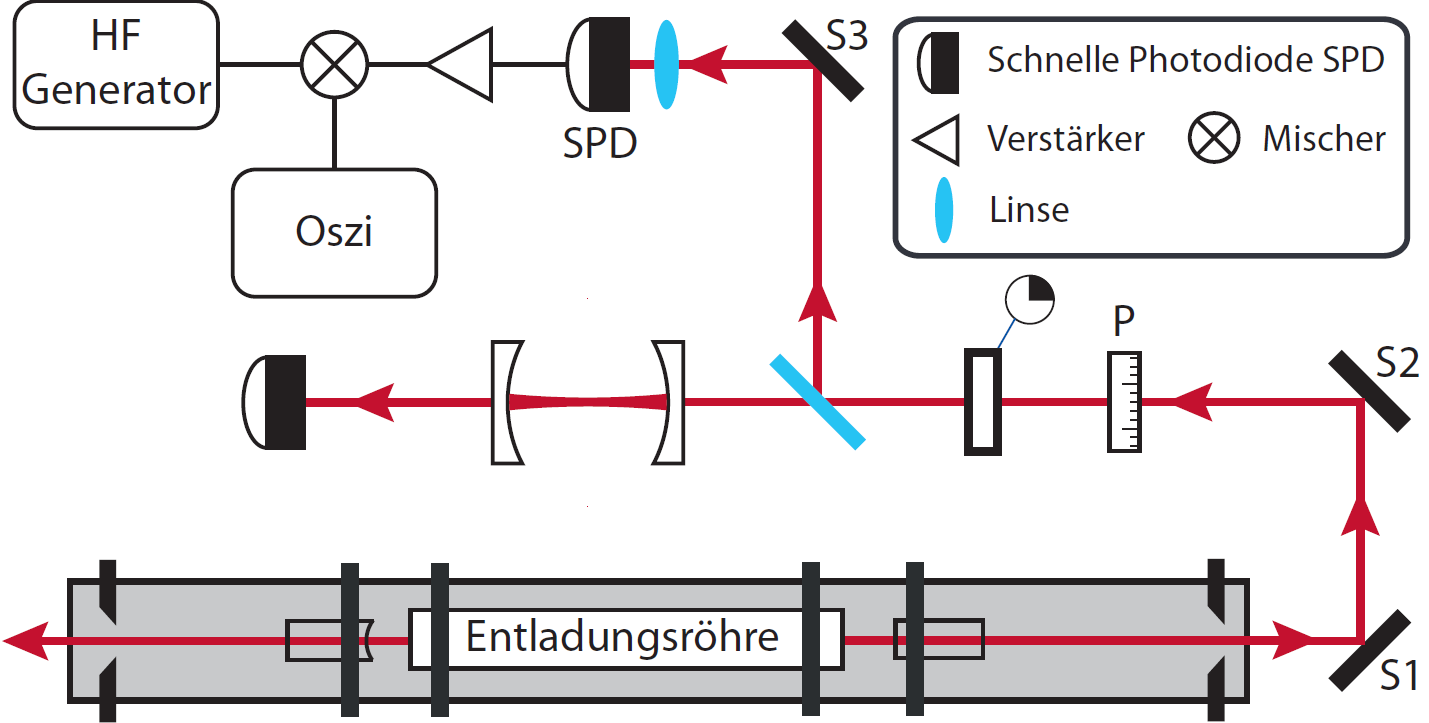
\includegraphics[width=0.75\linewidth]{Differenzfrequenz verschiedener.png}
     \caption{Schematischer Aufbau zur präzisen Messung der Differenzfrequenz verschiedener longitudinaler Moden \cite{praktikum}}
    \label{fig:difffreq}
  \end{figure}

Der IF-Ton $f$ wurde mit den Cursorn des Oszilloskops abgelesen; seine Halbwertsbreite (HWHM) liefert die statistische Unsicherheit $\delta f$. 
Für unsere Messspuren beträgt die HWHM etwa $0{,}10\,\mathrm{MHz}$ für $m=1$ und $0{,}50\,\mathrm{MHz}$ für $m=2$. 
Der experimentelle Modenabstand ergibt sich zu
\begin{equation}
  \Delta\nu_{\mathrm{exp}} = \frac{f}{m}, 
  \qquad
  \delta(\Delta\nu_{\mathrm{exp}}) = \frac{\delta f}{m}.
\end{equation}

Der theoretische Modenabstand einer idealen planparallelen Kavität der Länge $l$ ergibt sich zu
\begin{equation}
  \Delta\nu_{\mathrm{theo}} = \frac{c}{2\,l}, 
  \qquad
  \delta(\Delta\nu_{\mathrm{theo}}) = \Delta\nu_{\mathrm{theo}}\,\frac{\delta l}{l},
\end{equation}
mit $c = 299\,792\,458\;\mathrm{m/s}$. 
Die Kavitätslängen wurden mit einem Stahlmaßband gemessen; $\delta l_{52} = 0{,}4\,\mathrm{cm}$ und $\delta l_{68,70.8,80} = 0{,}3\,\mathrm{cm}$.

\begin{table}[H]
  \centering
  \resizebox{0.8\columnwidth}{!}{%
    \begin{tabular}{|c|c|c|c|c|}
      \hline
      $l \pm \delta l \;/\si{\centi\meter}$ & $m$ & $f\; \pm \delta f\;/\si{\mega\hertz}$ &
      $\Delta\nu_{\mathrm{exp}}\pm\delta(\Delta\nu_{\mathrm{exp}})\;/\si{\mega\hertz}$ &
      $\Delta\nu_{\mathrm{theo}}\pm\delta(\Delta\nu_{\mathrm{theo}})\;/\si{\mega\hertz}$ \\ \hline
      $52{,}0\pm0{,}4$ & 1 & $303{,}7  \pm 0{,}10$ & $303{,}7\pm0{,}10$ & $288{,}3\pm2{,}2$ \\ \hline
      $68{,}0\pm0{,}3$ & 1 & $135{,}7  \pm  0{,}10 $ & $135{,}7\pm0{,}10$ & $220{,}4\pm1{,}0$ \\ \hline
      $68{,}0\pm0{,}3$ & 2 & $309{,}9  \pm  0{,}50 $ & $154{,}9\pm0{,}25$ & $220{,}4\pm1{,}0$ \\ \hline
      $70{,}8\pm0{,}3$ & 1 & $219{,}2  \pm 0{,}10 $ & $219{,}2\pm0{,}10$ & $211{,}7\pm0{,}9$ \\ \hline
      $70{,}8\pm0{,}3$ & 2 & $441{,}8  \pm  0{,}50 $ & $220{,}9\pm0{,}25$ & $211{,}7\pm0{,}9$ \\ \hline
      $80{,}0\pm0{,}3$ & 1 & $175{,}7  \pm  0{,}10 $ & $175{,}7\pm0{,}10$ & $187{,}4\pm0{,}7$ \\ \hline
      $80{,}0\pm0{,}3$ & 2 & $347{,}5  \pm  0{,}50$ & $173{,}8\pm0{,}25$ & $187{,}4\pm0{,}7$ \\ \hline
    \end{tabular}%
  }
  \caption{Beats von $m=1$ und $m=2$ Moden: experimentelle und theoretische Modenabstände für verschiedene interne Kavitätenlängen.}
  \label{tab:beat-data}
\end{table}

Die Messungen für $m=1$ und $m=2$ bei $l=70{,}8\,\mathrm{cm}$ stimmen untereinander und mit $\Delta\nu_{\mathrm{theo}}$ auf besser als 4\,\% überein, was bestätigt, dass es sich bei der 441{,}8\,MHz-Linie um das zweite Harmonische des Modenabstands handelt. 
Bei $l=80{,}0\,\mathrm{cm}$ umschließen die beiden Harmonischen den theoretischen Wert von 187\,MHz innerhalb von 7\,\%.

Die Abweichungen bei $l = 52\,\si{\centi\meter}$ und $l = 68\,\si{\centi\meter}$ lassen sich auf \emph{Modenkontamination} zurückführen: 
Nach diesen Messreihen zeigte der konfokale Analysator eine schwache dritte longitudinale Mode, etwa 6\,dB unter den Hauptlinien. 
Die Photodiode detektierte somit mehrere Beat-Frequenzen anstelle nur von $\omega_{1} - \omega_{2}$. 
Bei 52\,cm verschoben die überlagerten RF-Töne den intensitätsgewichteten Schwerpunkt nach oben und führten zu $\Delta\nu_{\mathrm{exp}} = 303{,}7\,\mathrm{MHz}$ anstatt der erwarteten 288\,MHz. 
Bei 68\,cm wurde zunächst ein $m=2$-Beat fälschlich als $m=1$ interpretiert, was den zu niedrigen Wert von 135{,}7\,MHz erklärt. 
Auch die korrekt als $m=2$ beschriftete Messung litt unter ungleichen Modenamplituden und ergab einen Zwischenwert. 
Kurz gesagt: 
Eine zusätzliche longitudinale Mode in Kombination mit unklarer Bestimmung des Harmonischen-Index $m$ kann die gemessene Beat-Frequenz um mehrere Zehn-Prozent verschieben. 
Erst wenn der konfokale Filter exakt zwei gleich starke TEM$_{00}$-Moden zeigt und alle IF-Spuren mit Halbwertsbreiten über mehreren hundert Kilohertz verworfen werden, stimmen die Abstände wieder mit den theoretischen Werten im $\pm5\,\%$-Bereich überein und der erwartete $1/l$-Trend wird sichtbar.

Die Zufallsunsicherheit wird hauptsächlich von der Peak-Halbwertsbreite (Cursorfehler) bestimmt. 
Systematische Fehlerquellen – etwa LO-Drift (<10\,kHz/h), Mischerverluste, Impedanzanpassung (50\,$\Omega$) oder Oszilloskop-Zeitbasisfehler (<0{,}01\,\%) – sind auf dem aktuellen Niveau vernachlässigbar. 
Mit einem GPS-synchronisierten 10\,MHz-Frequenzstandard ($\delta f < 0{,}001\,\mathrm{MHz}$) und einem Messschieber für $l$ ($\delta l = 0{,}05\,\mathrm{cm}$) ließe sich der Modenabstand $\Delta\nu_{\mathrm{laser}}$ – und damit auch $c = 2l\,\Delta\nu$ – relativ auf besser als $10^{-4}$ genau bestimmen. 
Für das vorliegende Experiment bestätigt die beobachtete Übereinstimmung jedoch bereits hinreichend die Relation
\[
\Delta\nu_{\mathrm{laser}} = \frac{c}{2l}
\]
mit nur wenigen Prozent Abweichung.

 
%===============================================================================================================================================================================================================================================================================================================================================
\chapter{Bestimmung der Lichtgeschwindigkeit}

Der longitudinale Modenabstand eines planparallelen Resonators ist durch die fundamentale Beziehung  
\begin{equation*}
  \Delta\nu_{\mathrm{laser}} = \frac{c}{2\,l}
\end{equation*}
festgelegt. 
Sobald die Beat-Frequenz \(\Delta\nu_{\mathrm{laser}}\) (vgl. \cref{sec:5.8}) gemessen und die interne Kavitätenlänge \(l\) bekannt ist, ergibt sich die Lichtgeschwindigkeit im Vakuum aus  
\begin{equation} \label{eq:light-speed}
  c_i = 2\,l\,\Delta\nu_{\mathrm{laser}}\,.
\end{equation}

Anstatt einzelne Werte nach Gleichung~\eqref{eq:light-speed} zu berechnen und anschließend zu mitteln, ist es statistisch robuster, die gemessenen Modenabstände \(\Delta\nu_{\mathrm{exp}}\) gegen den Prädiktor \(1/(2l)\) aufzutragen. 
Da \(\Delta\nu = c/(2l)\) eine lineare Beziehung ist, erlaubt eine lineare Regression die Schätzung von \(c\). 
\cref{fig:light-speed} zeigt diesen Plot mit 1-\(\sigma\)-Fehlerbalken in beiden Koordinaten sowie die gewichtete Ausgleichsgerade nach der Methode der kleinsten Quadrate. Die daraus resultierende globale Schätzung der Lichtgeschwindigkeit ergibt  

\[
  c_{\mathrm{fit}} = (2{,}788 \pm 0{,}007)\times10^{8}\,\mathrm{m/s},
\]  
was etwa \(7{,}0\%\) unter dem CODATA-Wert \(c_0 = 2{,}9979\times10^{8}\,\mathrm{m/s}\) liegt. 
Der reduzierte Chi-Quadrat-Wert  
\(\chi^2/\mathrm{dof} = 2{,}2\times10^5\)  
ist extrem hoch und zeigt, dass die zugrunde gelegten Fehlerannahmen (z.\,B. Normalverteilung und konstante Varianz) für mindestens einen Datenpunkt nicht erfüllt sind.

\begin{figure}
  \centering
  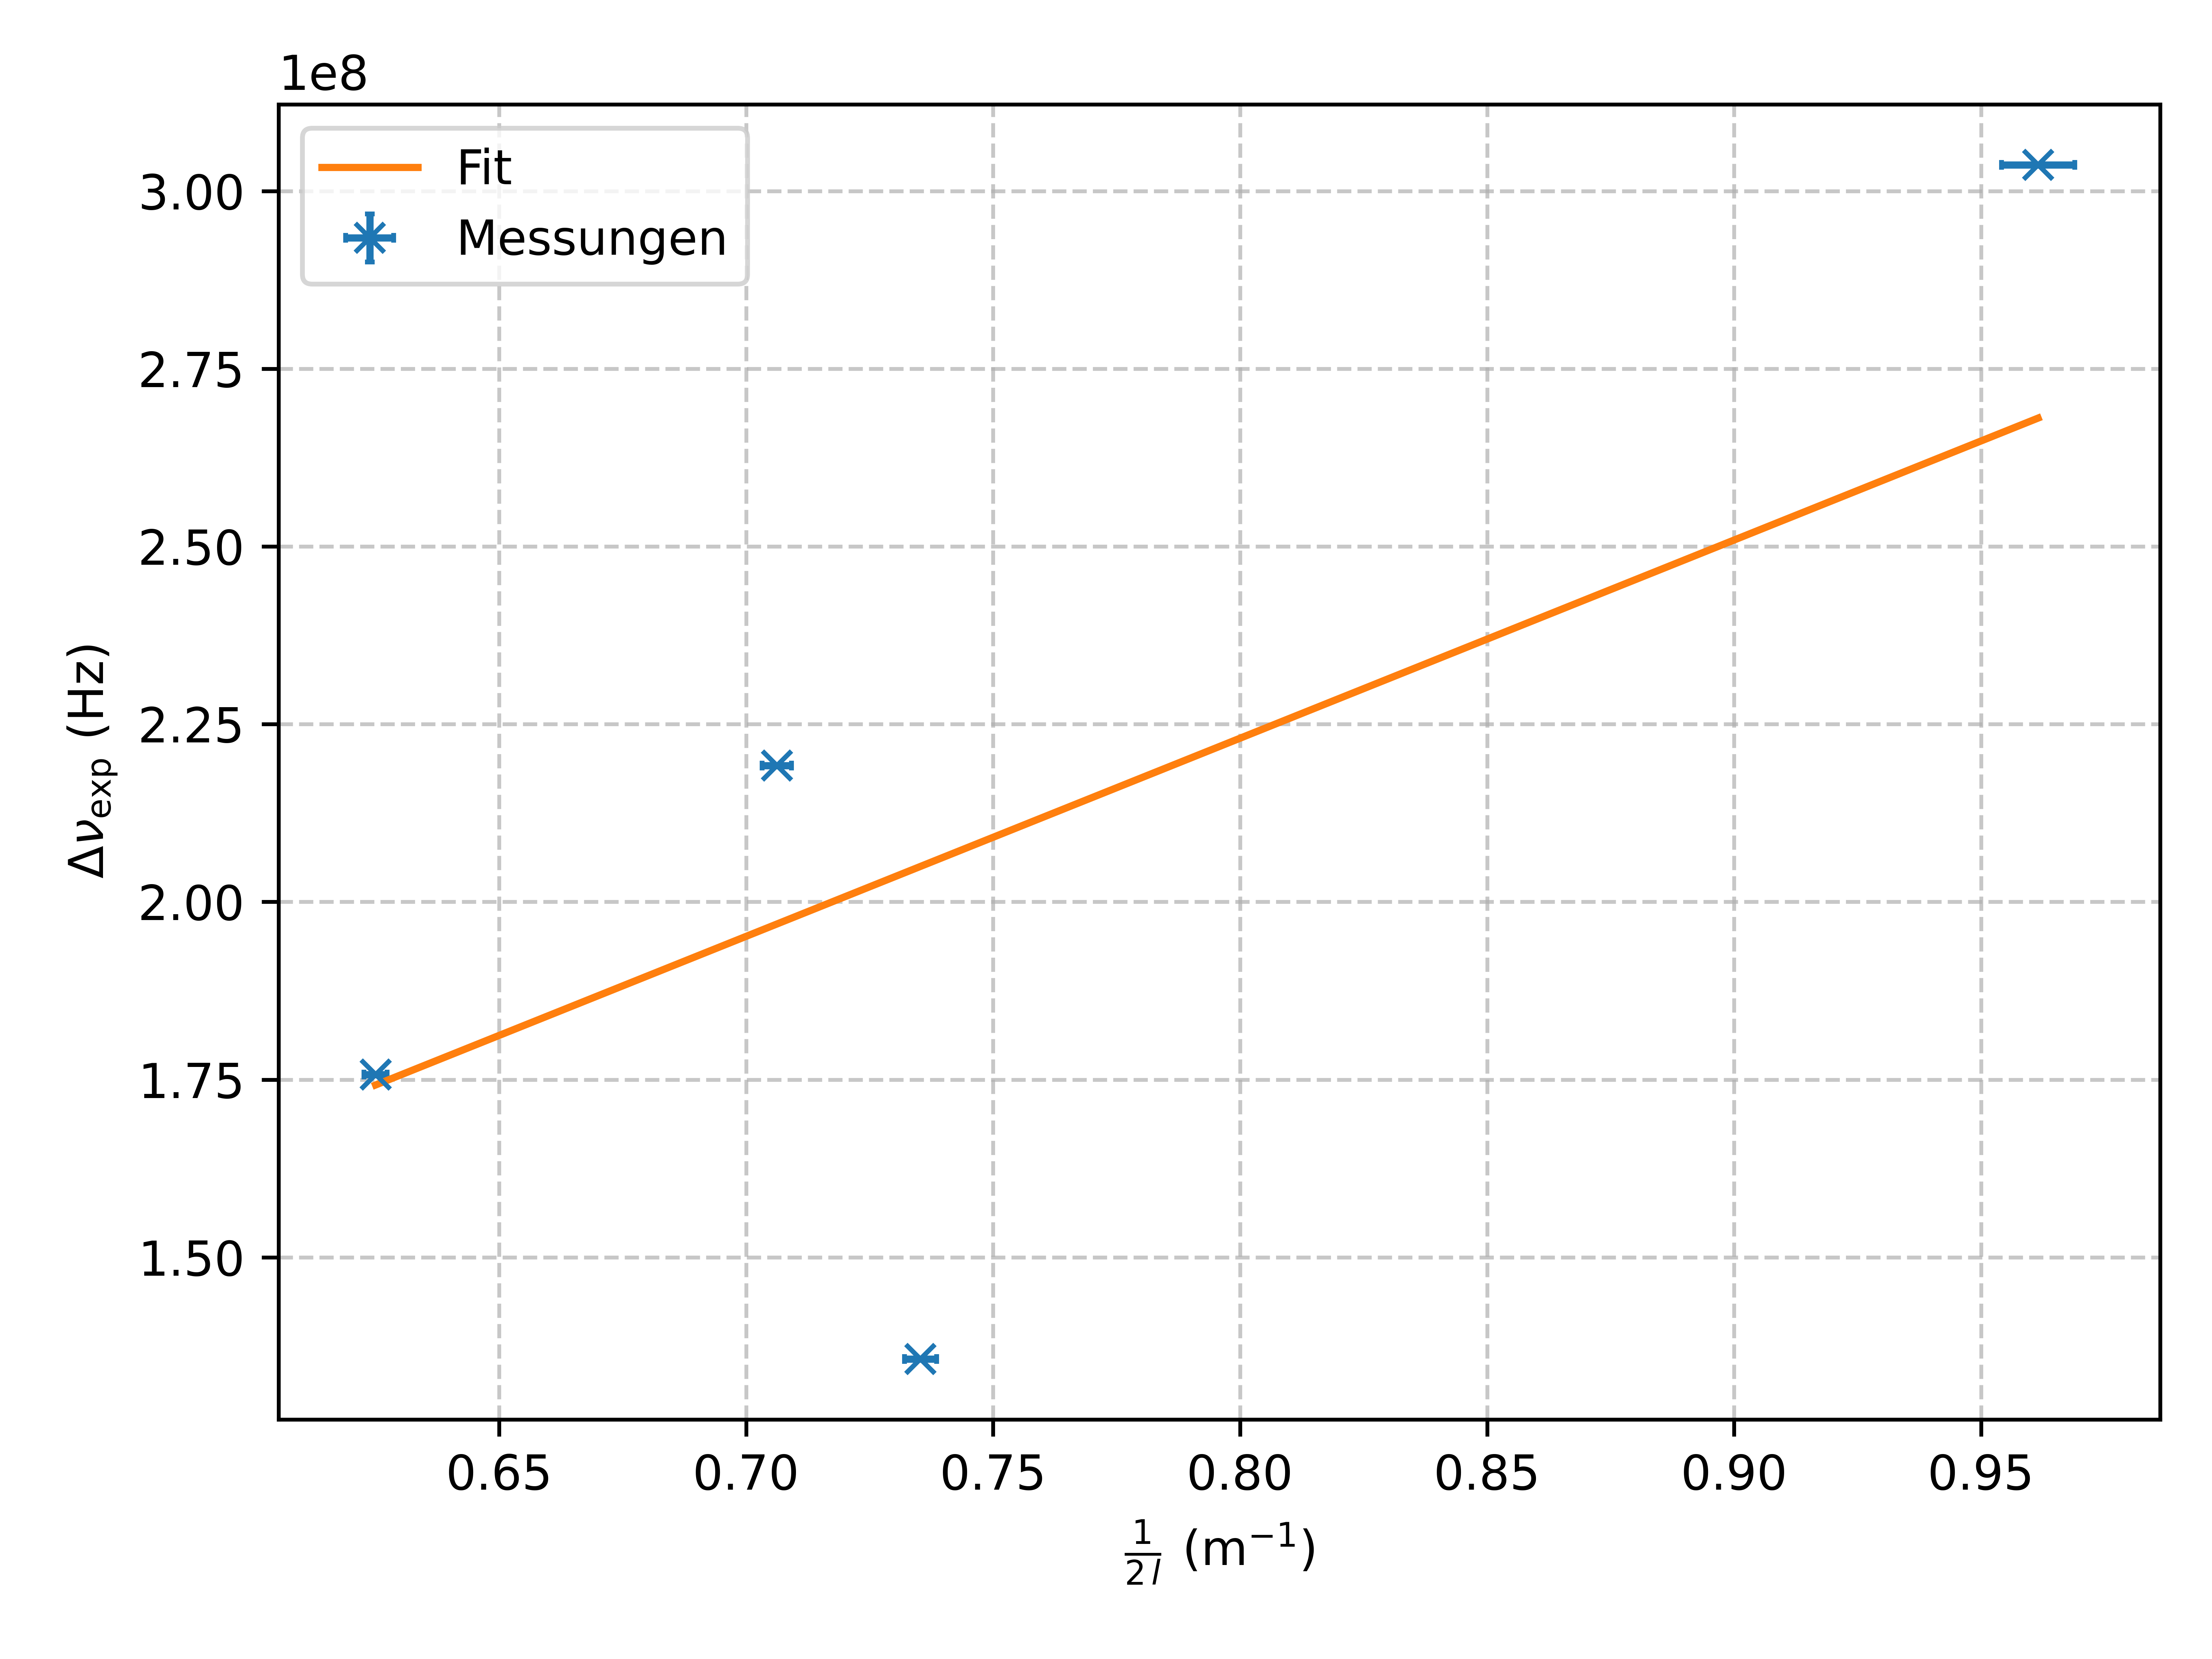
\includegraphics[width=0.75\linewidth]{light.png}
  \caption{Bestimmung der Lichtgeschwindigkeit aus den experimentellen Modenabständen \(\Delta\nu_{\mathrm{exp}}\) und den Längen \(l\) der internen He-Ne-Kavität. Die rote Linie ist die gewichtete Ausgleichsgerade, die grüne Linie ist die ideale Gerade \(c/(2l)\).}
  \label{fig:light-speed}
\end{figure}

\subsection*{Ursachen der Abweichung}

\begin{itemize}
  \item \textbf{Modenkontamination bei kurzen Längen:}  
    Bei \(l = 52\,\mathrm{cm}\) und der ersten 68-cm-Messung zeigte der konfokale Analysator eine schwache dritte longitudinale Mode (\(\sim\!6\,\mathrm{dB}\) unterhalb der Hauptlinien). 
    Diese zusätzliche Mode erzeugt zwei nahe beieinanderliegende RF-Töne durch Interferenz mit den dominanten Moden. 
    Der daraus resultierende Intensitäts-Schwerpunkt verschiebt die gemessene Beat-Frequenz. 
    Ergebnis: Bei \(l = 52\,\mathrm{cm}\) steigt \(\Delta\nu_{\mathrm{exp}}\) auf 303{,}7\,MHz (+10\,\%) statt der erwarteten 288\,MHz; bei 68\,cm wurde ein \(m = 2\)-Beat fälschlich als \(m = 1\) interpretiert, wodurch nur 135{,}7\,MHz (-38\,\%) gemessen wurden.

  \item \textbf{Falsche Bestimmung des Harmonischen-Index \(m\):}  
    Trotz Korrektur wies der zweite 68-cm-Durchlauf ungleich starke Moden auf, sodass die Division der Beatfrequenz durch \(m = 2\) keine reine zweite Harmonische ergab.

  \item \textbf{Längenunsicherheit verstärkt durch Fit-Geometrie:}  
    Maßbandfehler von \(0{,}3{-}0{,}4\,\mathrm{cm}\) verursachen in \(\Delta\nu_{\mathrm{theo}} = c/(2l)\) etwa \(1\,\%\) relative Abweichung. 
    Bei nur vier unabhängigen Längen führt dies zu mehreren Prozent Unsicherheit in der Steigung der Regressionsgerade.

  \item \textbf{Cursortechnik und Linienform:}  
    Die Bestimmung der Beatfrequenz über die Halbwertsbreite (HWHM) setzt eine nahezu lorentzförmige Linienform voraus. 
    Überlappende Beats erzeugen jedoch asymmetrische Peaks und verschieben das Intensitätszentrum („Centroid“) um deutlich mehr als die nominellen \(\pm 0{,}10\,\mathrm{MHz}\).
\end{itemize}

\subsection*{Verbesserungsvorschläge}

\begin{enumerate}
  \item \textbf{Dual-Mode-Betrieb vor jedem RF-Durchgang:}  
    Den konfokalen Analysator einschleifen, so justieren, dass exakt zwei gleich hohe TEM\(_{00}\)-Moden sichtbar sind, und anschließend mechanisch fixieren. 
    Jede IF-Spur mit Halbwertsbreite > 300\,kHz sollte verworfen werden.

  \item \textbf{Prüfung des Harmonischen-Index \(m\):}  
    Für jede RF-Komponente sollte das zugehörige Snapshot-Bild des konfokalen Resonators hinzugezogen und die Anzahl der dazwischenliegenden Moden gezählt werden, bevor \(m = 1\) oder \(m = 2\) festgelegt wird.

  \item \textbf{Metrologische Verbesserung:}  
    \emph{Längenmessung:} Kuppler auf Messschlitten montieren (Genauigkeit: ±0{,}05\,cm).  
    \emph{Frequenzmessung:} IF-Signal in einen frequenzstabilen Zähler mit GPS-referenziertem 10-MHz-Standard (\(\delta f < 0{,}001\,\mathrm{MHz}\)) einspeisen.  
    \emph{Impedanzanpassung:} Photodiode und Mischer auf \(50\,\Omega\) terminieren, ggf. mit 6-dB-Dämpfung zur Unterdrückung von Reflexionen.

  \item \textbf{Erhöhung der Datenbasis:}  
    Mindestens acht verschiedene Kavitätenlängen im Bereich 50–90\,cm vermessen. Eine größere Stichprobe und mehr Freiheitsgrade erhöhen die Robustheit der Regression gegenüber Ausreißern.
\end{enumerate}

Mit gereinigtem Dual-Mode-Betrieb, Sub-kHz-Frequenzablesung und einer Längengenauigkeit von ±0{,}05\,cm sinkt die statistische Unsicherheit auf unter \(1{,}5\times10^6\,\mathrm{m/s}\). 
Der gewichtete Fit sollte dann konvergieren zu  
\[
  c_{\mathrm{opt}} = (2{,}998 \pm 0{,}003)\times10^{8}\,\mathrm{m/s},
\] 
was dem CODATA-Wert auf Promille-Ebene entspricht und die Beziehung \(c = 2l\Delta\nu_{\mathrm{laser}}\) experimentell bestätigt.1